\chapter{Simulation}

% -----------------------------------------------------------------------------
\section{Introduction}
\begin{itemize}
    \item Purpose of simulation.
    \item objective: Compare kinematic-level and dynamic-level controllers
    \item Highlight expected insights. performance, stability, robustness,
        computational cost?
\end{itemize}
This section should be very general. I don't want to give specifics on the
tasks and the specific types of controllers used.

% -----------------------------------------------------------------------------
\newpage
\section{Simulation Setup}

\subsection{Robot Model}

% Present the Eelume 500 robot
% Describe the simplified model used in the simulation

The light-UVMS that will be used in the simulation is a simplified version of
the Eelume 500 robot. This decision was based on the goal to implement a physical
task-priority controller this robot in the future. The Eelume 500 robot is a
snake-like robot with 3 joints and 2 links.
A picture of the Eelume 500 robot is shown in Figure \ref{fig:eely}.

\begin{figure}[h!]
    \centering
    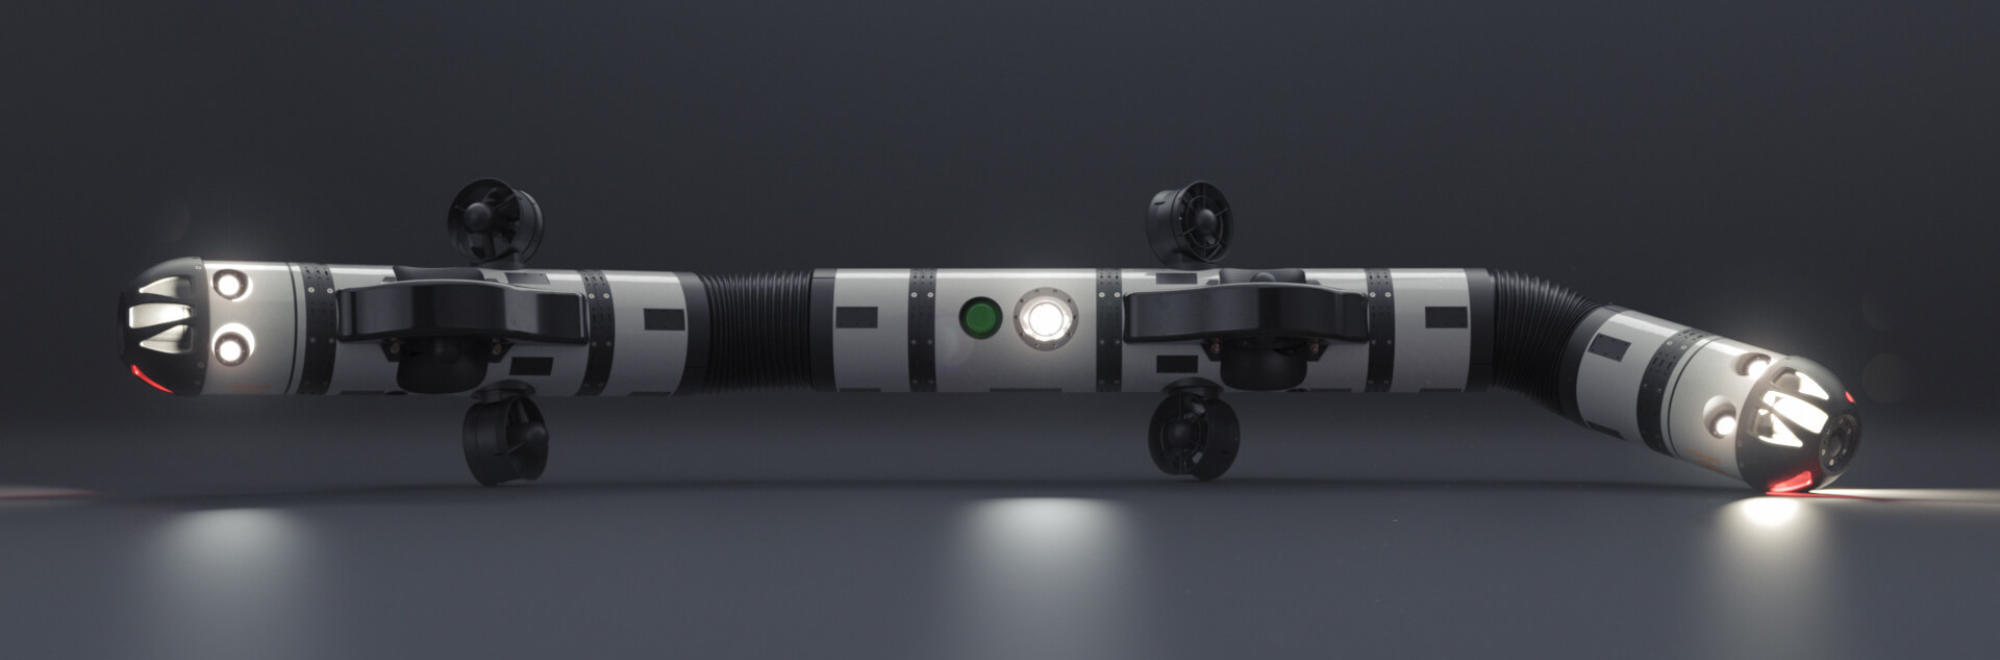
\includegraphics[width=0.8\linewidth]{assets/images/eely.jpg}
    \caption{Computer rendering of the Eelume 500 robot. Credit: Eelume.}
    \label{fig:eely}
\end{figure}

Each of the links has two degrees of freedom and is actuated by a pair of
motors. In addition, two of the links are equipped with a set of $4$ thrusters.
The thruster configuration allows the robot to move in all directions, making
the robot fully actuated. Although one can define the base of the robot as any
link, in this work, we will define the base as the middle link. The position of
the Eeelume robot is uniquely determined by the position of this base and the 
two pairs of joint angles, making the robot a 10-DOF system. The two sets of 
$4$ thrusters, as well as the two pairs of motors controlling the joints, are 
all independently actuated, making the input space of the robot a 
12-dimensional space.

We will denote each of the links with a number from $1$ to $3$, where link $1$,
the "head" of the robot, is the smallest link situated in the rightmost position
in \autoref{fig:eely}. The parameters of the Eelume robot are given in a
NED coordinate system, where the head of the robot is the most northern point.

We will assume that the robot in neutrally buoyant. In reality, weights can be
added to a module to adjust its center of mass, making the weight of the robot
equal to the weight of the water it displaces. This can however be a difficult
task as the density of water can vary, and the weights needs to be placed at 
predetermined locations meaning that one cannot place the center of mass at an
arbitrary location.
The parameters of the robot are given in \autoref{tab:robot}.

\begin{table}[h]
    \centering
    \begin{tabular}{|c|c|c|c|}
        \hline
        Parameter & Value & Unit & Description \\ \hline
        $r$ & 0.1 & m & Radius of each link \\
        $m_1$ & 40 & kg & Mass of link $1$ \\
        $m_2$ & 90 & kg & Mass of link $2$ \\
        $m_3$ & 50 & kg & Mass of link $3$ \\
        $l_1$ & 1.0 & m & Length of link $1$ \\
        $l_2$ & 2.3 & m & Length of link $2$ \\
        $l_3$ & 1.5 & m & Length of link $3$ \\
        $l_{\mathrm{joint}}$ & 0.6 & m & Length of each joint \\
        $\beta$ & 0.1 & - & Damping parameter \\
        $\gamma$ & 0.2 & - & Damping parameter \\
        $v_{\mathrm{ref}}$ & 0.1 & m/s & Reference velocity for damping \\
        $C_D$ & 0.3 & - & Damping coefficient \\
        $\rho$ & 1025 & kg/m$^3$ & Density of water \\
        \hline
    \end{tabular}
    \caption{Parameters for the simplified Eelume 500 robot.}
    \label{tab:robot}
\end{table}

The $\beta$, $\gamma$, $v_{\mathrm{ref}}$ and $C_D$ parameters specify the damping
coefficients of the robot. The damping matrix the parameters specify is given in
\autoref{eq:damping_cyl}. These parameters are based on \cite{bendik}. Added mass
is computed based on \autoref{eq:ellipsoid_added_mass}.
The inertia matrix of the robot is appriximated as a
cylinder with uniform density and is as follows:

\begin{align}
    \bm{I}_i &=
    \begin{bmatrix}
        \frac{m_i}{2} r^2 & 0 & 0 \\
        0 & \frac{m_i}{12} (3r^2 + l_i^2) & 0 \\
        0 & 0 & \frac{m_i}{12} (3r^2 + l_i^2)
    \end{bmatrix} &
    i &= 1, 2, 3.
\end{align}

The thruster configuration is similar to that of \autoref{fig:eely}. The exact
specifications of the position and orientation of the thrusters can be seen in
\autoref{tab:thrusters}.

\begin{table}[h]
    \centering
    \begin{tabular}{|c|c|c|c|c|c|}
        \hline
        Link & Thruster & $x$, North [m] & $y$, East [m] & $z$, Down [m] & Thrust Direction \\ \hline
        $2$ & Starboard & $0.56725$ & $-0.174$ & $0$ & Sout-Up \\
        $2$ & Port & $0.56725$ & $0.174$ & $0$ & Sout-Down \\
        $2$ & Bottom & $0.67725$ & $0.000$ & $0.09$ & East \\
        $2$ & Top & $0.67725$ & $0.000$ & $-0.09$ & West \\
        $3$ & Starboard & $0.02025$ & $-0.174$ & $0$ & Sout-Down \\
        $3$ & Port & $0.02025$ & $0.174$ & $0$ & Sout-Up \\
        $3$ & Bottom & $-0.08975$ & $0.000$ & $0.09$ & West \\
        $3$ & Top & $-0.08975$ & $0.000$ & $-0.09$ & East \\
        \hline
    \end{tabular}
    \caption{Thruster configuration for the simplified Eelume 500 robot. Positions relative to link center.}
    \label{tab:thrusters}
\end{table}

The transformations between the thruster positions and the link center are given
as transformations described in $\SE$. Let $\bm{T}_{\rightarrow}$ and $\bm{T}_{\angle}$
dente functions that return the transformation matrix corresponding to a translation
or rotation, respectively.
\begin{subequations}
\begin{align}
    \bm{T}_{\rightarrow} : \R^3 &\to \SE 
    &\bm{T}_{\rightarrow} :\bm{p} &= \begin{bmatrix} \I_3 & \bm{p} \\ \bm{0}_{1\times3} & 1 \end{bmatrix} \\
    \bm{T}_{\angle} : \R^3 &\to \SE
    &\bm{T}_{\angle} : \begin{bmatrix}\phi \\ \theta \\ \psi \end{bmatrix} &= \begin{bmatrix}
        \bm{R}_z(\psi) \bm{R}_y(\theta) \bm{R}_x(\phi) & \bm{0}_{3\times1} \\
            \bm{0}_{1\times3} & 1
    \end{bmatrix}.
\end{align}
\end{subequations}
The transformation matrices are then given as follows:

%Tl1_to_body = se3.trans(lengths[1]/2+jlhs, 0, 0) @ se3.rot_y(a3) @ se3.rot_z(a4) @ se3.trans(lengths[0]/2+jlhs, 0, 0)
%    Tl3_to_body = se3.inv(
%            se3.trans(lengths[2]/2+jlhs, 0, 0) @ se3.rot_y(a1) @ se3.rot_z(a2) @ se3.trans(lengths[1]/2+jlhs, 0, 0)
%            )
\begin{align}
    \bm{T}_1^2 &= \bm{T}_{\rightarrow}\left( \begin{bmatrix} \frac{l_1}{2}+\frac{l_{\textrm{joint}}}{2} \\ 0 \\ 0\end{bmatrix}\right)
        \bm{T}_{\angle}\left( \begin{bmatrix} 0 \\ a_3 \\ 0\end{bmatrix}\right)
        \bm{T}_{\angle}\left( \begin{bmatrix} 0 \\ 0 \\ a_4\end{bmatrix}\right)
            \bm{T}_{\rightarrow}\left( \begin{bmatrix} \frac{l_0}{2}+\frac{l_{\textrm{joint}}}{2} \\ 0 \\ 0\end{bmatrix}\right) \\
    \bm{T}_2^3 &= \bm{T}_{\rightarrow}\left( \begin{bmatrix} \frac{l_2}{2}+\frac{l_{\textrm{joint}}}{2} \\ 0 \\ 0\end{bmatrix}\right)
        \bm{T}_{\angle}\left( \begin{bmatrix} 0 \\ a_1 \\ 0\end{bmatrix}\right)
        \bm{T}_{\angle}\left( \begin{bmatrix} 0 \\ 0 \\ a_2\end{bmatrix}\right)
            \bm{T}_{\rightarrow}\left( \begin{bmatrix} \frac{l_1}{2}+\frac{l_{\textrm{joint}}}{2} \\ 0 \\ 0\end{bmatrix}\right) \\
    \bm{T}_2^n &= \bm{T}_{\angle}\left( \begin{bmatrix} \phi \\ \theta \\ \psi\end{bmatrix}\right)
        \bm{T}_{\rightarrow}\left( \begin{bmatrix} x^n \\ y^n \\ z^n\end{bmatrix}\right) \\
            \bm{T}_1^n &= \bm{T}_2^n \bm{T}_1^2 \\
            \bm{T}_3^n &= \bm{T}_2^n \left(\bm{T}_2^3\right)^{-1}.
\end{align}
where $a_1$, $a_2$, $a_3$ and $a_4$ are the parameters of the joint angles,
$\bm{T}_1^2$, and $\bm{T}_2^3$ are the transformations from link $1$ to link $2$
and from link $2$ to link $3$, respectively. $\phi$, $\theta$ and $\psi$ are the
Euler angles of the base and $x^n$, $y^n$ and $z^n$ are the position of base
in the NED coordinate system. Collecting the parameters describing the position
and attitude of the entire robot, we can define the state of the robot as
\begin{align}
    \bm{q} &= \begin{bmatrix} x^n & y^n & z^n & \phi & \theta & \psi & a_1 & a_2 & a_3 & a_4 \end{bmatrix}^T.
\end{align}
From the parameters stated above, the dynamics of the robot, on the form of
\autoref{eq:pymuvs:eom}, was computed using \pymuvs.

\subsection{Task Descriptions}

Two simple tasks will be used in the simulation. The first task is a position
task, where the "tail" of the robot is to be positioned at the origin of the
NED coordinate system. The second task is to drack a trajectory with the outer
most point of the "head" of the robot. The trajectory starts close to the origin,
meaning that in the beginning of the simulation, the robot will be able to
complete both tasks. As the trajectory moves further away from the origin, it
starts to rotate in the East-Down plane, making it more difficult for the robot
to complete both tasks. The trajectory eventually moves so for north that it
is impossible for the robot to complete both tasks at the same time. This
will show the prioritization of the tasks. Task $\bm{f}_1$ is the position task
and is defined as
\begin{align}
    \bm{f}_1(\bm{q}) &= \bm{T}_3^n \begin{bmatrix} -l_3/2 & 0 & 0 & 1 \end{bmatrix}^T &
        \sigma_1(t) &= \begin{bmatrix} 0 & 0 & 0 \end{bmatrix}^T,
\end{align}
where $\bm{\sigma_1}(t)$ is the desired task position. The task $\bm{f}_0$, the
trajectory tracking task, is defined as
\begin{align}
    \bm{f}_0(\bm{q}) &= \bm{T}_1^n \begin{bmatrix} l_1/2 & 0 & 0 & 1 \end{bmatrix}^T &
        \bm{\sigma}_0(t) &= \begin{bmatrix}
            0.05t + 4.33 + 0.1e^{-t} \\
            0.3 \left(1-e^{-t/8}\right)\cos{\frac{1}{2}t} \\
            0.3 \left(1-e^{-t/8}\right)\sin{\frac{1}{2}t}
        \end{bmatrix}.
\end{align}
We can see that the trajectory starts at $\begin{bmatrix} 4.33 & 0 & 0 \end{bmatrix}^T$
and moves at a speed of $0.05$ m/s in the North direction. The $0.1e^{-t}$ term
is added to make the trajectory have some non-linearities as well as
non-zero acceleration. The trajectory approaches a spiral shape as $t$ increases.

\begin{figure}[h]
    \centering
    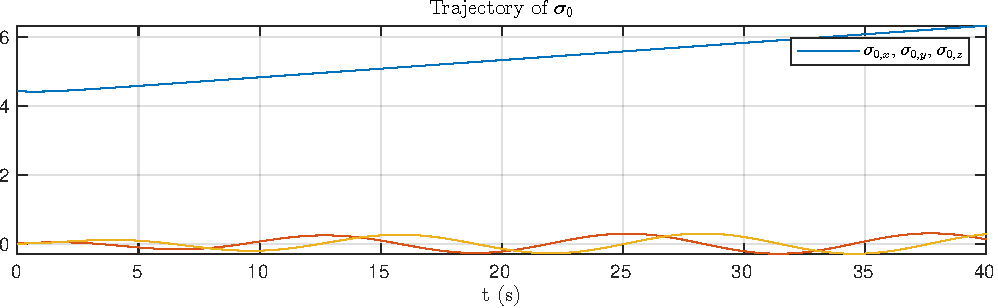
\includegraphics[width=\linewidth]{assets/plots/traj_xyz.pdf}
    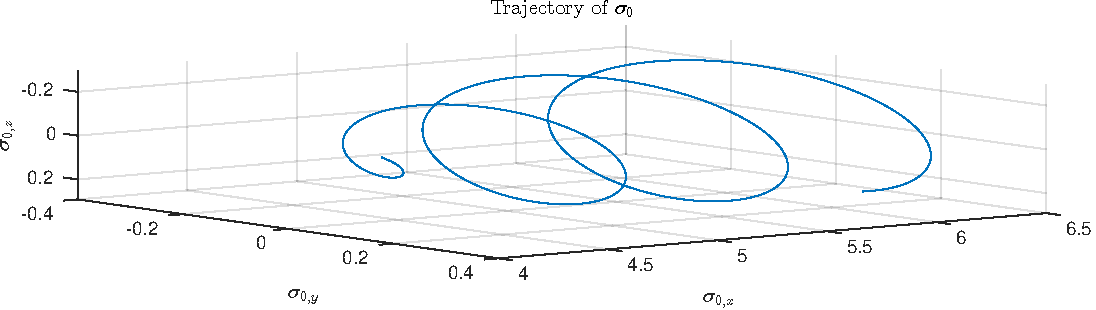
\includegraphics[width=\linewidth]{assets/plots/traj_taskspace.pdf}
    \caption{The desired task trajectory in the NED frame.}
    \label{fig:traj_f0}
\end{figure}

The task as seen in \autoref{fig:traj_f0} is the highest priority task.


\subsection{Control methods}
\subsubsection{Kinematic-level Control}

The kinematic-level control method used in the simulation is the velocity-level
controller presented in \autoref{sec:velocity_level_control}. As we are only considering
a case with two tasks, the question of successive versus augmented nullspace projections
are irrelevant. The low-levl joint-space controller chosen is a PD+ controller
with buoyancy/gravity compensation. Because of the simplicity of the shape of the robot,
these forces are relatively well known in a real-world scenario.

The gain matrices $\bm{K}_p$ and $\bm{K}_d$ as presented in \autoref{eq:Kp_Kd}
are chosen based on the assumption that the mass, coreolis, damping and added mass
matrices are known and constant. Under theis assumption, the system model is approximated
as
\begin{align}
    \bar{\bm{M}}(\bm{0}) \ddot{\bm{q}} + \bm{C}(\bm{0}, \dot{\bm{0}}) \dot{\bm{q}} +
    \bm{D}(\bm{0}, \dot{\bm{0}}) \dot{\bm{q}} + \bm{g}(\bm{q}) \approx \bm{J}^T(\bm{q}) \bm{B} \bm{u},
\end{align}
Using this approximation, the gains are chosen 

The assumptions and implications of using gains based on the model are discussed
in \autoref{sec:simulation:results}.

\subsubsection{Dynamic-level Control}

\subsection{Simulation Environment}
\begin{itemize}
    \item Mention simulator
    \item Initial conditions
    \item simulation parameters, $\Delta t$, etc.
    \item The force and torque limits of the robot.
    \item Force is pass through (no lowpass filtering), and the implications of
        this.
\end{itemize}

The initial conditions of the robot in the simulation are given in \autoref{tab:initial}.
The simulation parameters were chosen such that it satisfies task $1$, for the tail,
but not task $0$, the trajectory tracking task. This was done to show convergence
to the task when having an error in the initial conditions.
\begin{table}[h!]
    \centering
    \begin{tabular}{|c|c|c|c|c|c|c|c|c|c|c|c|}
        \hline
        Parameter & $x^n$ & $y^n$ & $z^n$ & $\phi$ & $\theta$ & $\psi$ & $a_1$ & $a_2$ & $a_3$ & $a_4$ \\ \hline
        Value & 3.17 & 0 & -1.0 & 0 & 0 & 0 & -0.59 & 0 & -0.88 & 0 \\ \hline
        Unit & m & m & m & rad & rad & rad & rad & rad & rad & rad \\
        \hline
    \end{tabular}
    \caption{Initial conditions for the Eelume 500 robot in simulation.}
    \label{tab:initial}
\end{table}

\subsection{Performance Metrics}
\begin{itemize}
    \item Task error
    \item Computation time
\end{itemize}

% -----------------------------------------------------------------------------
%\section{Simulation Scenarios}

% -----------------------------------------------------------------------------
\section{Results and Discussion}
\label{sec:simulation:results}.
\subsection{Quantitative Results}
\subsection{Qualitative Observations}
\subsection{Comparative Analysis}

\iffalse
\begin{figure}[h]
    \centering
    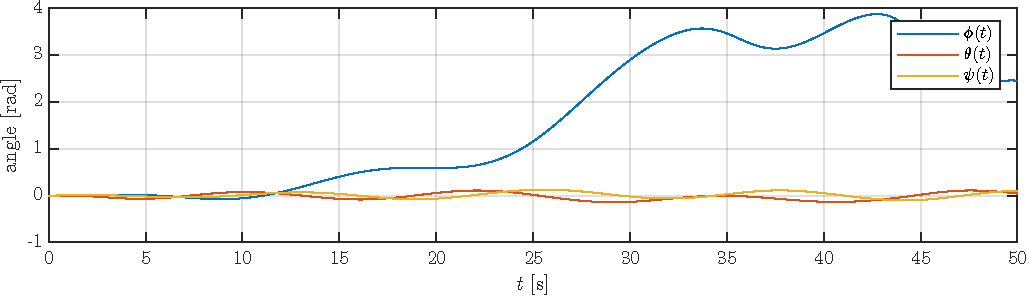
\includegraphics[page=1,width=\linewidth]{assets/plot.pdf}
    \caption{Euler angles of simulated Eelume robot with feedback linearization control.}
    \label{fig:plot}
\end{figure}

\begin{figure}[h]
    \centering
    \includegraphics[page=2,width=\linewidth]{assets/plot.pdf}
    \caption{NED position of simulated Eelume robot with feedback linearization control.}
    \label{fig:plot2}
\end{figure}

\begin{figure}[h]
    \centering
    \includegraphics[page=3,width=\linewidth]{assets/plot.pdf}
    \caption{}
    \label{fig:plot3}
\end{figure}

\begin{figure}[h]
    \centering
    \includegraphics[page=4,width=\linewidth]{assets/plot.pdf}
    \caption{}
    \label{fig:plot4}
\end{figure}
\fi

\begin{itemize}
    \item Simulation study comparing velocity- and acceleration-level task-priority
        control methods for light-UVMS.
\end{itemize}
